\chapter{Diffusion multiple par les défauts : matrice $T$ et taux d'amortissement}\label{chap:T}

Le chapitre précédent a construit la matrice de couplage électron-défaut $M$ à partir des premiers principes et ce chapitre l'utilise pour calculer le taux d'amortissement électronique dû aux défauts. À cet effet, nous développons la théorie de la perturbation à plusieurs corps appliquée au couplage électron-défaut. Nous commençons par le cas le plus simple d'un seul défaut, pour lequel le problème se résout exactement dans le formalisme de la matrice $T$~\cite{bruusManyBodyQuantumTheory2004} (section~\ref{sec:mbt_T}), puis généralisons à un grand nombre de défauts répartis aléatoirement (section~\ref{sec:mbt_sigma}). Les quantités mesurables par l'expérience ne dépendent pas de la réalisation microscopique du désordre et sont plutôt des moyennes sur les positions des défauts, que la théorie de la perturbation permet d'évaluée dans la limite diluée. La matrice $T$ est ensuite résolue en exploitant sa localisation dans l'espace réel, rendue manifeste par les fonctions de Wannier, à faible coût numérique sur des grilles arbitrairement denses (section~\ref{sec:T_local}). Les sections~\ref{sec:T_détails} et~\ref{sec:T_results} donnent les paramètres du calcul et les résultats pour des lacunes dans le graphène.

\section{Un défaut et la matrice $T$}\label{sec:mbt_T}

Commençons par le cas idéal où il n'y a qu'un seul défaut présent dans le matériau et ignorons toutes les autres perturbations. Supposons que le problème électronique a été résolu par la DFT dans le système parfait. Le couplage entre les électrons du système et le défaut se fait par l'entremise de l'Hamiltonien de couplage électron-défaut, et nous travaillons maintenant à température finie c'est-à-dire dans l'ensemble grand canonique, de sorte que l'Hamiltonien du système est
\begin{equation}
    \hat{H}-\mu\hat{N} = \hat{H}_\text{e}+\hat{H}_\text{ed} = \sum_{n\kv}\xi_{n\kv}\hat{c}^\dag_{n\kv}\hat{c}_{n\kv}+\sum_{nm}\sum_{\kv\kv'}M_{mn}(\kv',\kv)\hat{c}^\dag_{m\kv'}\hat{c}_{n\kv},\quad\xi_{n\kv} \equiv \varepsilon_{n\kv}-\mu
\end{equation}
où la matrice $M_{mn}(\kv',\kv)=\matrixel{\psi_{m\kv'}}{V_\text{ed}(\rv)}{\psi_{n\kv}}$ représente physiquement l'amplitude de probabilité qu'un électron dans l'état $\ket{\psi_{n\kv}}$ diffuse vers l'état $\ket{\psi_{m\kv'}}$ via le potentiel $V_\text{ed}(\rv)$ induit par le défaut dans le matériau, $\xi_{n\kv}\equiv\varepsilon_{ n\kv}-\mu$ et $\mu$ est le potentiel chimique. Nous souhaitons employer la méthode de la théorie de la perturbation pour résoudre ce problème. Notre objectif est de déterminer la fonction de Green de Matsubara à température finie ; une fois celle-ci calculée, la grande majorité des propriétés physiques mesurables peuvent être extraites de cette fonction. Dans le formalisme de Matsubara, nous travaillons avec un temps imaginaire $\tau\in[0,\beta]$, où $\beta=1/k_BT$ est l'inverse de la température et la fonction de Green est généralement calculée dans la représentation d'interaction en mécanique quantique~\cite{mahanManyParticlePhysics2000}
\begin{equation}
    \mathcal{G}_{mn}(\tau'-\tau) = -\frac{{}_0\langle\mathcal{T}_\tau\hat{c}_m(\tau')S(\beta,0)\hat{c}
    _n^\dag(\tau)\rangle_0}{{}_0\langle S(\beta,0)\rangle_0}.\label{eqn:G_formel}
\end{equation}
Ici, les indices $m$ et $n$ de l'équation~\eqref{eqn:G_formel} sont des indices composés de bande et de vecteur d'onde, $m\equiv(m\kv')$ et $n\equiv(n\kv)$, ${}_0\langle\dots\rangle_0$ est une moyenne thermique par rapport à l'Hamiltonien non perturbé $\hat{H}_\text{e}$, $\mathcal{T}_\tau$ est l'opérateur d'ordonnancement dans le temps imaginaire, la dépendance en temps imaginaire des opérateurs $\hat{O}(\tau)$ est obtenue dans la représentation de l'interaction (donc déterminée par $\hat{H}_\text{e}$) et la matrice $S(\beta, 0)$ inclut les effets de couplage entre les électrons et le défaut et est définie formellement par
\begin{equation}
    S(\beta, 0) = \mathcal{T}_\tau\exp[-\int_0^\beta d\tau\,\hat{H}_\text{ed}(\tau)] = \sum_{p=0}^\infty\frac{(-1)^p}{p!}\int_0^\beta d\tau_1\dots\int_0^\beta d\tau_p\mathcal{T}_\tau\left[\hat{H}_\text{ed}(\tau_1)\cdots\hat{H}_\text{ed}(\tau_p)\right].\label{eqn:S}
\end{equation}
Pour calculer la fonction de Green de l'équation~\eqref{eqn:G_formel}, nous devons développer la matrice $S$ à l'aide de l'équation~\eqref{eqn:S} puis évaluer les moyennes thermiques. Comme ces moyennes sont faites par rapport à l'Hamiltonien libre $\hat{H}_\text{e}$, qui est quadratique dans les opérateurs de création et d'annihilation, elles peuvent être évaluées avec le théorème de Wick. Cependant, cette approche souffre du même problème que l'application de la théorie de la perturbation dans le cadre de la spectroscopie Raman : il n'est pas trivial d'énumérer tous les termes qui découlent du développement de la matrice $S$. Pour remédier à ce problème, nous employons à nouveau des diagrammes de Feynman, avec les règles de la figure~\ref{fig:règles_Raman}. En théorie, nous devons développer la matrice $S$ au numérateur et au dénominateur de l'équation~\eqref{eqn:G_formel} simultanément, ce qui devient rapidement problématique. En pratique, le théorème des amas connexes (de l'anglais \textit{linked-cluster theorem}) stipule que les diagrammes engendrés par le développement de la matrice $S$ au dénominateur annulent exactement les diagrammes déconnectés du développement au numérateur. Cela simplifie considérablement la tâche. Toute cette machinerie est présentée en détail dans l'annexe~\ref{annexe:défauts} et nous reprenons seulement les étapes importantes ici.

Le résultat central de cette annexe est que la fonction de Green de Matsubara pour des électrons en interaction avec un seul défaut satisfait une équation de Dyson qui est illustrée diagrammatiquement dans la figure~\ref{fig:G_Dyson}.
\begin{center}
    \vspace{0.5\baselineskip}
    % Vertex électron-défaut : cercle blanc + croix (cf. tikz/règles_Raman.tex)
\providecommand{\vertexdefaut}[1]{%
  \draw[fill=white] (#1) circle (0.2);
  \draw[line width=1pt] ($(#1)+(-0.14,-0.14)$) -- ($(#1)+(0.14,0.14)$);
  \draw[line width=1pt] ($(#1)+(-0.14,0.14)$) -- ($(#1)+(0.14,-0.14)$);
}

% Extrémités d'un terme : #1 x gauche, #2 x droit
\providecommand{\bornesserie}[2]{%
  \fill (#1,0) circle (0.05);
  \fill (#2,0) circle (0.05);
  \node[below=2pt] at (#1,0) {\small$\tau$};
  \node[below=2pt] at (#2,0) {\small$\tau'$};
}

\begin{tikzpicture}[
    line/.style={thick},
    >=Stealth,
    fermion/.style={
      postaction={decorate},
      decoration={markings, mark=at position 0.55 with {\arrow{Stealth}}}
    },
]

\node[anchor=east] at (1.55,0) {$\mathcal{G}_{mn}(\tau'-\tau) =$};

% ---- ordre 0 : propagation libre ----
\draw[line, fermion] (1.75,0) -- (2.90,0);
\bornesserie{1.75}{2.90}

\node at (3.25,0) {$+$};

% ---- ordre 1 : un vertex ----
\draw[line, fermion] (3.60,0) -- (4.18,0);
\draw[line, fermion] (4.58,0) -- (5.16,0);
\vertexdefaut{4.38,0}
\bornesserie{3.60}{5.16}

\node at (5.51,0) {$+$};

% ---- ordre 2 : deux vertex ----
\draw[line, fermion] (5.86,0) -- (6.44,0);
\draw[line, fermion] (6.84,0) -- (7.42,0);
\draw[line, fermion] (7.82,0) -- (8.40,0);
\vertexdefaut{6.64,0}
\vertexdefaut{7.62,0}
\bornesserie{5.86}{8.40}

\node at (8.75,0) {$+$};

% ---- ordre 3 : trois vertex ----
\draw[line, fermion] (9.10,0)  -- (9.68,0);
\draw[line, fermion] (10.08,0) -- (10.66,0);
\draw[line, fermion] (11.06,0) -- (11.64,0);
\draw[line, fermion] (12.04,0) -- (12.62,0);
\vertexdefaut{9.88,0}
\vertexdefaut{10.86,0}
\vertexdefaut{11.84,0}
\bornesserie{9.10}{12.62}

\node[anchor=west] at (12.95,0) {$+\ \cdots$};

\end{tikzpicture}

    \captionof{figure}{Équation de Dyson pour la fonction de Green de Matsubara électronique en présence d'un défaut.}
    \label{fig:G_Dyson}
    \vspace{0.5\baselineskip}
\end{center}
Cette équation de Dyson est plus généralement réécrite en employant la matrice $T$ dans le contexte de la diffusion sur des défauts. Cette matrice $T$ est définie diagrammatiquement à la figure~\ref{fig:T_matrice} et joue un rôle similaire à la \textit{self}-énergie électronique.
\begin{center}
    \vspace{0.5\baselineskip}
    % Définition diagrammatique de la matrice T : développement complet (première
% ligne) et forme récursive de Dyson (deuxième ligne).
% Style identique aux diagrammes du chapitre Raman (tikz/e1.tex, tikz/pd.tex).
% Compatible pdflatex. Requiert : tikz, decorations.markings, arrows.meta, calc.
% Le blob hachuré est tracé à la main (clip + traits) pour éviter d'avoir à
% charger la bibliothèque patterns dans le préambule.

% Vertex électron-défaut : cercle blanc + croix (cf. tikz/règles_Raman.tex)
\providecommand{\vertexdefaut}[1]{%
  \draw[fill=white] (#1) circle (0.2);
  \draw[line width=1pt] ($(#1)+(-0.14,-0.14)$) -- ($(#1)+(0.14,0.14)$);
  \draw[line width=1pt] ($(#1)+(-0.14,0.14)$) -- ($(#1)+(0.14,-0.14)$);
}

% Matrice T : cercle hachuré. #1 = coordonnée du centre.
\providecommand{\blobT}[1]{%
  \begin{scope}
    \clip (#1) circle (0.28);
    \foreach \i in {-8,...,8} {
      \draw[line width=0.4pt] ($(#1)+(0.08*\i-0.45,-0.45)$) -- ($(#1)+(0.08*\i+0.45,0.45)$);
    }
  \end{scope}
  \draw[thick, fill=none] (#1) circle (0.28);
}

\begin{tikzpicture}[
    line/.style={thick},
    >=Stealth,
    fermion/.style={
      postaction={decorate},
      decoration={markings, mark=at position 0.55 with {\arrow{Stealth}}}
    },
]

% ============ première ligne : développement complet ============
\node[anchor=east] at (1.5,0) {$T_{mn} \equiv$};
\blobT{1.9,0}
\node at (2.6,0) {$=$};

% un vertex
\vertexdefaut{3.3,0}
\node at (3.9,0) {$+$};

% deux vertex
\vertexdefaut{4.5,0}
\draw[line, fermion] (4.7,0) -- (5.7,0);
\vertexdefaut{5.9,0}
\node at (6.5,0) {$+$};

% trois vertex
\vertexdefaut{7.1,0}
\draw[line, fermion] (7.3,0) -- (8.3,0);
\vertexdefaut{8.5,0}
\draw[line, fermion] (8.7,0) -- (9.7,0);
\vertexdefaut{9.9,0}
\node[anchor=west] at (10.35,0) {$+\ \cdots$};

% ============ deuxième ligne : forme récursive ============
\node at (2.6,-1.7) {$=$};

\vertexdefaut{3.3,-1.7}
\node at (3.9,-1.7) {$+$};

\vertexdefaut{4.5,-1.7}
\draw[line, fermion] (4.7,-1.7) -- (5.72,-1.7);
\blobT{6.0,-1.7}

\end{tikzpicture}

    \captionof{figure}[Expression diagrammatique de la matrice $T$ pour la diffusion sur un seul défaut.]{Expression diagrammatique de la matrice $T$ pour la diffusion sur un seul défaut. La première ligne donne le développement complet, la deuxième la forme récursive.}
    \label{fig:T_matrice}
    \vspace{0.5\baselineskip}
\end{center}
À l'aide de la matrice $T$, l'équation de Dyson pour la fonction de Green prend la forme donnée diagrammatiquement à la figure~\ref{fig:dyson_T}.
\begin{center}
    \vspace{0.5\baselineskip}
    % Série de Dyson resommée en termes de la matrice T :
%   G_{mn}(tau'-tau) = G^(0) + G^(0) T G^(0)
% Style identique aux diagrammes du chapitre Raman (tikz/e1.tex, tikz/pd.tex).
% Compatible pdflatex. Requiert : tikz, decorations.markings, arrows.meta, calc.
%
% Convention temporelle : temps croissant de gauche à droite, donc
% tau < tau_1 < tau_2 < tau'. Le deuxième terme se lit
%   G^(0)_m(tau'-tau_2) T_{mn}(tau_2-tau_1) G^(0)_n(tau_1-tau).
% Si l'équation du texte adopte l'ordre inverse, il suffit d'échanger les
% étiquettes tau_1 et tau_2 ci-dessous.

% Vertex électron-défaut : cercle blanc + croix (cf. tikz/règles_Raman.tex)
\providecommand{\vertexdefaut}[1]{%
  \draw[fill=white] (#1) circle (0.2);
  \draw[line width=1pt] ($(#1)+(-0.14,-0.14)$) -- ($(#1)+(0.14,0.14)$);
  \draw[line width=1pt] ($(#1)+(-0.14,0.14)$) -- ($(#1)+(0.14,-0.14)$);
}

% Matrice T : cercle hachuré. Définition identique à celle de tikz/matrice_T.tex.
\providecommand{\blobT}[1]{%
  \begin{scope}
    \clip (#1) circle (0.28);
    \foreach \i in {-8,...,8} {
      \draw[line width=0.4pt] ($(#1)+(0.08*\i-0.45,-0.45)$) -- ($(#1)+(0.08*\i+0.45,0.45)$);
    }
  \end{scope}
  \draw[thick, fill=none] (#1) circle (0.28);
}

\begin{tikzpicture}[
    line/.style={thick},
    >=Stealth,
    fermion/.style={
      postaction={decorate},
      decoration={markings, mark=at position 0.55 with {\arrow{Stealth}}}
    },
]

\node[anchor=east] at (1.55,0) {$\mathcal{G}_{mn}(\tau'-\tau) =$};

% ---- premier terme : propagateur libre ----
\draw[line, fermion] (1.75,0) -- (3.35,0);
\node[above=3pt] at (2.55,0) {$n$};
\fill (1.75,0) circle (0.05);
\fill (3.35,0) circle (0.05);
\node[below=2pt] at (1.75,0) {\small$\tau$};
\node[below=2pt] at (3.35,0) {\small$\tau'$};

\node at (3.85,0) {$+$};

% ---- deuxième terme : G^(0) T G^(0) ----
\draw[line, fermion] (4.35,0) -- (5.95,0);
\node[above=3pt] at (5.15,0) {$n$};
\blobT{6.23,0}
\node[above=8pt] at (6.23,0) {$T_{mn}$};
\draw[line, fermion] (6.51,0) -- (8.11,0);
\node[above=3pt] at (7.31,0) {$m$};

\fill (4.35,0) circle (0.05);
\fill (8.11,0) circle (0.05);
\node[below=2pt] at (4.35,0) {\small$\tau$};
% étiquettes splayées en biais : les deux points d'attache du blob ne sont
% distants que de 0.56, insuffisant pour deux étiquettes centrées
\node[anchor=north east] at (5.99,-0.10) {\small$\tau_1$};
\node[anchor=north west] at (6.47,-0.10) {\small$\tau_2$};
\node[below=2pt] at (8.11,0) {\small$\tau'$};

\end{tikzpicture}

    \captionof{figure}[Série de Dyson pour la fonction de Green en présence d'un seul défaut, via la matrice $T$.]{Série de Dyson pour la fonction de Green de Matsubara électronique en présence d'un seul défaut, exprimée en fonction de la matrice $T$. Les temps $\tau_1$ et $\tau_2$ sont intégrés.}
    \label{fig:dyson_T}
    \vspace{0.5\baselineskip}
\end{center}
En traduisant ces diagrammes à l'aide des règles de Feynman, la matrice $T$ de la figure~\ref{fig:T_matrice} s'écrit
\begin{equation}
    T = M + M\mathcal{G}^{(0)}T,\label{eqn:T_chap}
\end{equation}
où les produits sont matriciels sur les indices $(n\kv)$ et convolutifs en temps imaginaire, et la fonction de Green de la figure~\ref{fig:dyson_T} devient
\begin{equation}
    \mathcal{G} = \mathcal{G}^{(0)}+\mathcal{G}^{(0)}T\mathcal{G}^{(0)}.\label{eqn:G_chap}
\end{equation}
Les convolutions en temps imaginaire se démêlent dans l'espace des fréquences de Matsubara fermioniques $i\omega_j$, défini à l'annexe~\ref{annexe:défauts} dans l'équation~\eqref{eqn_G_tau}, où elles deviennent de simples produits. La quantité $\mathcal{G}^{(0)}$ est la fonction de Green de Matsubara pour le système non perturbé, soit en l'absence de défauts. Elle est connue analytiquement et prend la forme
\begin{equation}
    \mathcal{G}^{(0)}_{n\kv}(i\omega_j) = \frac{1}{i\omega_j-\xi_{n\kv}}.
\end{equation}
Comme le défaut est statique, $M$ ne dépend pas de la fréquence et l'équation~\eqref{eqn:T_chap} se résout par une inversion de matrice à chaque fréquence
\begin{equation}
    T(i\omega_j) = \left[\mathbb{I}-M\mathcal{G}^{(0)}(i\omega_j)\right]^{-1}M.
\end{equation}
Une fois la matrice $T$ calculée, nous pouvons calculer la fonction de Green qui prend la forme explicite
\begin{equation}
    \mathcal{G}_{mn}(\kv',\kv;i\omega_j) =\delta_{mn}\delta_{\kv\kv'}\mathcal{G}^{(0)}_{n\kv}(i\omega_j)+\mathcal{G}_{m\kv'}^{(0)}(i\omega_j)T_{mn}(\kv',\kv; i\omega_j)\mathcal{G}_{n\kv}^{(0)}(i\omega_j),
\end{equation}
dans l'espace des fréquences de Matsubara. Notons que nous avons ici une expression analytique \textit{exacte} pour la fonction de Green : le problème est résolu exactement. Ceci ne devrait pas être trop surprenant, car il s'agit d'un problème à un corps. Notons également que le formalisme de la matrice $T$ inclut les effets du défaut sur les électrons à tous les ordres de la théorie de la perturbation. Cela est particulièrement intéressant pour les défauts considérés dans ce mémoire, les lacunes, qui induisent un potentiel de défaut si fort qu'il n'est pas justifié de tronquer la série de Dyson à un ordre fini. Le formalisme de la matrice $T$ demeure valide dans tous les régimes de force de potentiel de défaut.
Enfin, notons que les quantités physiques mesurables sont les fonctions dites \textit{retardées}, définies
sur l'axe des fréquences réelles, tandis que nous avons des expressions pour les quantités sur l'axe des fréquences imaginaires. Les quantités retardées s'obtiennent des fonctions de Matsubara par prolongement analytique, $i\omega_j \to \omega + i\eta$ avec $\eta \to 0^+$, qui est ici une simple substitution puisque nous disposons d'expressions analytiques fermées (voir la discussion sur la continuation analytique à la fin de l'annexe~\ref{annexe:défauts}). Généralement, les fonctions retardées sont identifiées par un exposant $R$. Or, dans tout ce mémoire, les quantités définies sur l'axe des fréquences réelles sont implicitement retardées et l'exposant $R$ est supprimé.

La connaissance de la fonction de Green retardée dans l'espace des fréquences réelles nous donne accès à la densité d'états
\begin{equation}
    \rho(\omega) = -\frac{1}{\pi}\mathrm{Im}\,\mathrm{Tr}\,\mathcal{G}(\omega).\label{eqn:rho}
\end{equation}
En utilisant l'équation pour la fonction de Green~\eqref{eqn:G_chap}, la variation de la densité d'états induite par un défaut s'écrit
\begin{align}
    \delta\rho(\omega) &= -\frac{1}{\pi}\,\mathrm{Im}\,\mathrm{Tr}\!\left[\mathcal{G}^{(0)}T\mathcal{G}^{(0)}\right]\\
    &= \frac{1}{\pi}\,\mathrm{Im}\,\mathrm{Tr}\!\left[T(\omega)\frac{\partial\mathcal{G}^{(0)}}{\partial\omega}\right],\label{eqn:delta_rho}
\end{align}
où nous avons utilisé $\partial\mathcal{G}^{(0)}/\partial \omega = -(\mathcal{G}^{(0)})^2$ et la propriété cyclique de la trace. Elle est exprimée en états par unité d'énergie et par défaut. Elle est positive là où le défaut crée des états et négative là où il en retire. Enfin, elle satisfait la règle de somme
\begin{equation}
    \int d\omega\,\delta\rho(\omega) = 0,
\end{equation}
c'est-à-dire que le défaut déplace les états sans en changer le nombre.

\section{Plusieurs défauts et la \textit{self}-énergie}\label{sec:mbt_sigma}

Bien que le formalisme de la matrice $T$ offre une solution exacte au problème de l'interaction entre les électrons d'un matériau et un seul défaut, n'importe quel matériau réaliste contient un très grand nombre de défauts. En effet, un matériau peut être pur à une partie par milliard ($10^9$) ; pour une quantité macroscopique de ce matériau ($10^{23}$ atomes), cela représente tout de même $10^{14}$ défauts. Nous devons donc généraliser au cas où il y a $N_d$ lacunes réparties aléatoirement dans le matériau. Le potentiel induit par cette collection de défauts est maintenant
\begin{equation}
    V_\text{ed}(\rv) = \sum_{I=1}^{N_d}V_\text{ed}(\rv-\rv_I),
\end{equation}
où $V_\text{ed}(\rv-\rv_I)$ est le potentiel induit par la lacune à la position $\rv_I=\Rv_\ell+\bm\tau_\alpha$, de sorte que $I=(\alpha\ell)$ est un indice composé (ici encore $\ell$ identifie les cellules unitaires du matériau et $\alpha$ identifie les atomes dans une cellule unitaire). Puisque ce potentiel dépend de la position des défauts, il va de soi que la fonction de Green résultante dépend aussi de la position des défauts. En d'autres mots, les propriétés microscopiques du matériau dépendent de la réalisation exacte du désordre. Cependant, les propriétés macroscopiques mesurées par l'expérience (par exemple, la densité d'états, le spectre de quasi-particules ou bien l'intensité Raman) sont insensibles à la réalisation particulière du désordre : elles correspondent à la moyenne sur toutes les configurations de positions $\{\rv_I\}$ possibles, notée $\overline{\mathcal{G}}\equiv\langle\mathcal{G}\rangle_{\{\rv_I\}}.$ Cette moyenne sur les positions des lacunes restaure la symétrie de translation du système, brisée par chaque configuration individuelle, de sorte que $\overline{\mathcal{G}}$ est diagonale en $\kv$ et s'écrit sous la forme d'une équation de Dyson habituelle~\cite{mahanManyParticlePhysics2000}
\begin{equation}
    \overline{\bm{\mathcal{G}}}_{\kv}(\omega) = \left[\left(\bm{\mathcal{G}}^{(0)}_{\kv}(\omega)\right)^{-1}-\bm{\Sigma}_{\kv}^\text{ed}(\omega)\right]^{-1},\label{eqn:G_moyenne}
\end{equation}
où $\bm{\Sigma}_{\kv}^\text{ed}$ est la \textit{self}-énergie électronique due aux défauts. Si la moyenne restaure la symétrie de translation, elle ne diagonalise pas la \textit{self}-énergie dans l'indice de bande. Le potentiel des lacunes couple toujours les bandes entre elles : $\overline{\bm{\mathcal{G}}}_{\kv}$, $\bm{\mathcal{G}}^{(0)}_{\kv}$ et $\bm{\Sigma}^\text{ed}_{\kv}$ sont des matrices dans cet indice et l'inverse est matriciel. Seule la fonction de Green non perturbée est toujours diagonale en bande : $\mathcal{G}^{(0)}_{mn\kv}(\omega)=\delta_{mn}[\omega-\xi_{n\kv}]^{-1}$. Contrairement au cas d'un défaut unique, cette moyenne ne peut pas être effectuée exactement, d'où l'utilité de la théorie de la perturbation. En suivant la même procédure qui conduit à l'expression analytique pour $\mathcal{G}$, nous obtenons une expansion perturbative pour la \textit{self}-énergie en série de puissances de la concentration de défauts $c\equiv N_d/N_\text{uc}$. Ce calcul n'est pas répété ici et le lecteur intéressé peut consulter le chapitre 11 de l'ouvrage de Bruus et Flensberg~\cite{bruusManyBodyQuantumTheory2004}.

Dans ce mémoire, nous travaillons dans la limite diluée, $c\ll 1$, où les processus de diffusion sur des défauts différents sont indépendants les uns des autres. Cette limite couvre toutes les concentrations de défauts expérimentalement pertinentes : pour le graphène, une concentration de l'ordre de $c\sim 1~\%$ correspond à une densité de défauts de $\sim 2\times 10^{13}$ cm$^{-2}$, qui est un échantillon de piètre qualité. Les processus de diffusion impliquant $p$ défauts distincts sont d'ordre $c^p$ et sont supprimés pour $p>1$ dans cette limite. Ainsi, la \textit{self}-énergie se réduit, au premier ordre en $c$, à la somme des diffusions multiples sur chaque défaut pris isolément, ce qui correspond précisément à la matrice $T$ de la section~\ref{sec:mbt_T}, évaluée sur sa diagonale en $\kv$ et multipliée par le nombre de défauts~\cite{bruusManyBodyQuantumTheory2004}
\begin{equation}
    \Sigma_{mn\kv }^\text{ed}(\omega) = N_d T_{mn}(\kv,\kv;\omega)+\mathcal{O}(c^2).\label{eqn:sigma_diluée}
\end{equation}
Cette approximation où la \textit{self}-énergie est proportionnelle à la matrice $T$, appelée Born complète (de l'anglais \textit{full Born approximation}) et aussi connue sous le nom de l'approximation de la matrice $T$, est exacte au premier ordre en concentration et demeure valide quelle que soit la force du potentiel de défaut.

Pour simplifier les calculs, nous ne retenons que la partie diagonale en bande de la matrice, $T_{n\kv}(\omega)\equiv T_{nn}(\kv,\kv;\omega)$, de sorte que la \textit{self}-énergie est elle aussi diagonale en bande $\Sigma^\text{ed}_{n\kv}=N_dT_{n\kv}$ et la fonction de Green moyennée pour plusieurs défauts prend la forme habituelle
\begin{equation}
    \overline{\mathcal{G}}_{n\kv}(\omega)=\left[\omega-\xi_{n\kv}-\Sigma^\text{ed}_{n\kv}\right]^{-1}.\label{eqn:G_moyenne_diag}
\end{equation}
Ceci est une autre approximation. Elle se justifie néanmoins en trois temps. D'abord, une lacune sur un site du sous-réseau A et une lacune sur un site du sous-réseau B produisent des éléments hors-diagonaux opposés entre les bandes $\pi$ et $\pi^*$ au voisinage des points $K$ et $K'$. Pour une distribution aléatoire de défauts également répartis sur les deux sous-réseaux comme nous le supposons, ces éléments s'annulent \textit{en moyenne}. Ensuite, entre les bandes non dégénérées, l'effet des éléments hors-diagonaux résiduels sur le spectre est d'ordre $|\Sigma^\text{ed}_{mn}|^2/|\xi_{m\kv}-\xi_{n\kv}|$ (obtenu au deuxième ordre dans la théorie de la perturbation ordinaire). Avec des \textit{self}-énergies de quelques dizaines de meV aux concentrations désirées (voir la section~\ref{sec:T_results}) et des séparations de bandes de l'ordre de l'eV, cet effet est négligeable. Enfin, aux points de dégénérescence $\pi/\pi^*$ où cet argument perturbatif échoue ($\xi_{\pi K}-\xi_{\pi^*K}=0$), la quantité que nous rapportons à la section~\ref{sec:T_results} est la demi-trace du bloc dégénéré, invariante sous sa diagonalisation et seule la répartition de l'amortissement au sein de la paire dépend de l'approximation. Le traitement complet de la structure en bande de la \textit{self}-énergie est laissé en perspective.

Le membre de droite de l'équation~\eqref{eqn:sigma_diluée} est intensif : avec la convention de la section~\ref{sec:M_détails}, les états de Bloch sont normalisés sur la cellule unitaire et le facteur $1/N_\text{uc}$ qui accompagne la normalisation sur le cristal fait de $N_dT$ une quantité proportionnelle à $c$, qui est finie dans la limite thermodynamique. Nous rapportons donc les résultats dans la section~\ref{sec:T_results} sous la forme $\Sigma/c$, indépendante de la concentration.

Une fois que la matrice $T$ est calculée en suivant les développements de la section~\ref{sec:mbt_T} et que le prolongement analytique est effectué, la \textit{self}-énergie s'obtient directement dans l'espace des fréquences réelles (c'est une quantité retardée) par une simple multiplication par un scalaire suivant l'équation~\eqref{eqn:sigma_diluée}. Cette \textit{self}-énergie se décompose en une partie réelle et une partie imaginaire
\begin{equation}
    \Sigma_{n\kv}^\text{ed}(\omega) = \Sigma_{n\kv}^{\text{ed}'}(\omega) + i\Sigma_{n\kv}^{\text{ed}''}(\omega).
\end{equation}
La partie réelle $\Sigma_{n\kv}^{\text{ed}'}$ renormalise l'énergie des bandes et la partie imaginaire $\Sigma_{n\kv}^{\text{ed}''}$ définit le taux d'amortissement dû aux défauts
\begin{equation}
\Gamma_{n\kv}^{\text{ed}} = -2\Sigma_{n\kv}^{\text{ed}''}.
\end{equation}
C'est ce taux d'amortissement, avec son homologue pour le couplage électron-phonon et pour les phonons advenant le cas où il y a un phonon créé dans l'état intermédiaire, qui fixe l'élargissement des états électroniques intermédiaires dans les dénominateurs résonants des amplitudes Raman du chapitre~\ref{chap:Raman}. Le temps de vie électronique dû aux défauts est relié au taux d'amortissement par
\begin{equation}
    \tau^\text{ed}_{n\kv} = \frac{\hbar}{\Gamma^\text{ed}_{n\kv}} = -\frac{\hbar}{2\Sigma^{\text{ed}\prime\prime}_{n\kv}}.
\end{equation}

Il est instructif de situer notre traitement dans la hiérarchie des approximations usuelles pour la \textit{self}-énergie de désordre~\cite{elliottTheoryPropertiesRandomly1974}. Premièrement, l'approximation de Born tronque la série pour la matrice $T$ à ses deux premiers termes, de sorte que la \textit{self}-énergie s'écrit
\begin{equation}
    \Sigma_{n\kv}^\text{ed,B}\approx N_d[M+M\mathcal{G}^{(0)}M].
\end{equation}
Cette approximation, qui ignore les diffusions multiples sur un même défaut, n'est pas valable dans la limite où les potentiels induits par les défauts sont forts, comme c'est le cas pour les lacunes. Nous quantifions cet échec dans la section~\ref{sec:T_results}. Ensuite, nous avons l'approximation de Born complète (ou de la matrice $T$), qui inclut les diffusions multiples sur un même défaut à tous les ordres et est l'approximation dans laquelle nous travaillons. La \textit{self}-énergie prend la forme
\begin{equation}
    \Sigma_{n\kv}^{\text{ed,T}}\approx N_dT_{n\kv},
\end{equation}
et est exacte au premier ordre en concentration des défauts, quelle que soit la force du potentiel. Ensuite, l'approximation de la matrice $T$ autocohérente (SCTA, de l'anglais \textit{Self-Consistent $T$-matrix Approximation})~\cite{klauderModificationElectronEnergy1961,peresElectronicPropertiesDisordered2006} va un cran plus loin en calculant la matrice $T$ avec la fonction de Green moyennée $\overline{\mathcal{G}}$ plutôt qu'avec la fonction de Green non perturbée $\mathcal{G}^{(0)}$. Cela donne trois équations couplées à résoudre de manière autocohérente
\begin{equation}
    \Sigma_{n\kv}^\text{ed,SCTA} = N_d\overline{T}_{n\kv},\quad \overline{T} = M+M\overline{\mathcal{G}}\overline{T},\quad \overline{\mathcal{G}}_{n\kv} = \left[\omega-\xi_{n\kv}-\Sigma_{n\kv}^\text{ed,SCTA} \right]^{-1}.
\end{equation}
La SCTA inclut la rétroaction de l'élargissement de désordre sur la diffusion elle-même et apporte des corrections d'ordre $\mathcal{O}(c^2)$, donc négligeables dans la limite diluée, sauf au voisinage immédiat des points de Dirac du graphène où la densité d'états est nulle et l'autocohérence engendre une densité d'états finie induite par le désordre~\cite{peresElectronicPropertiesDisordered2006}. Les états électroniques intermédiaires pertinents pour la double résonance Raman se trouvent à plusieurs dixièmes d'eV du point de Dirac pour la lumière visible utilisée dans les expériences de spectroscopie Raman : les corrections apportées par la SCTA sont négligeables ici et nous les laissons en perspective. Enfin, au-delà de ces approximations à un site, l'approximation du potentiel cohérent (CPA, de l'anglais \textit{Coherent Potential Approximation})~\cite{sovenCoherentPotentialModelSubstitutional1967} et l'inclusion de diagrammes croisés reliant plusieurs défauts deviennent nécessaires aux concentrations élevées ou pour les propriétés de transport cohérent, que nous ne considérons pas ici.

Dans la limite diluée de cette section, les défauts contribuent indépendamment à la densité d'états, et celle du matériau désordonné est
\begin{equation}
    \rho(\omega) = \rho_0(\omega) + c\delta\rho(\omega),
\end{equation}
où $\rho_0$ est la densité d'états du matériau parfait.

\section{Schéma de l'amas pour la matrice $T$}\label{sec:T_local}

La résolution directe de l'équation~\eqref{eqn:T_chap} requiert une inversion dans la base complète des états de Bloch et n'est pas possible sur les grilles ultra denses requises pour la convergence de l'intensité Raman (nous quantifions cet argument dans la section~\ref{sec:T_détails}). La localisation de la matrice de couplage dans l'espace réel permet de contourner cette limitation. En effet, la section~\ref{sec:M_results} montre que, dans la base des fonctions de Wannier, les éléments $M_{ij}(\Rv',\Rv)$ sont négligeables dès que $\Rv$ ou $\Rv'$ s'éloigne de la lacune. Or, en itérant l'équation récursive~\eqref{eqn:T_chap} pour la matrice $T$, elle s'écrit
\begin{equation}
    T = M+ M\mathcal{G}^{(0)}M+M\mathcal{G}^{(0)}M\mathcal{G}^{(0)}M+\dots,
\end{equation}
dont chaque terme est multiplié à gauche et à droite par $M$ : la matrice $T_{ij}(\Rv',\Rv)$, dans cette base, est donc elle aussi négligeable dès que $\Rv$ ou $\Rv'$ s'éloigne de la lacune. L'idée est donc de restreindre les calculs au sous-ensemble des cellules unitaires où $M$ n'est pas négligeable : le sous-espace dit \textit{local}. Il suffit alors de travailler avec les $N_L$ cellules situées à distance $R\le R_\text{cut}$ de la lacune, recentrée à l'origine, où $R$ est la norme euclidienne des indices réduits de la maille et $R_\text{cut}$ est le même rayon de coupure que celui introduit pour l'interpolation de $M$. La base est alors de dimension $N_LN_W$, où $N_W=5$ est le nombre de fonctions de Wannier, et est indépendante de la grille dense sur laquelle les quantités seront finalement évaluées. Nous appelons $M_\text{loc}$ la matrice de couplage restreinte à ce sous-espace et $g^{(0)}$ la fonction de Green du système non perturbé restreinte de la même façon. Dans ce sous-espace, l'équation~\eqref{eqn:T_chap} devient
\begin{equation}
    t(\omega) = M_\text{loc}\left[\mathbb{I}-g^{(0)}(\omega)M_\text{loc}\right]^{-1},\label{eqn:t_loc}
\end{equation}
et requiert une inversion de dimension $N_LN_W$, beaucoup plus facile que l'inversion directe de l'équation~\eqref{eqn:T_chap} et ce, peu importe la densité de la grille de sortie. Cette réécriture est essentiellement exacte si $R_\text{cut}$ englobe toutes les cellules où $M$ est non négligeable.

Il est important de souligner que $g^{(0)}$ est la fonction de Green du système infini, dont nous ne gardons que les éléments entre les fonctions de Wannier voisines de la lacune. Ce n'est pas la fonction de Green d'un morceau fini de graphène. Elle s'écrit, dans la base des fonctions de Wannier
\begin{equation}
g^{(0)}_{ij}(\Rv',\Rv;\omega) = \frac{1}{N_{\tilde\kv}}\sum_{\tilde \kv} e^{i\tilde\kv\cdot(\Rv'-\Rv)}\left[(\omega+i\eta)\mathbb{I}-H(\tilde\kv)\right]^{-1}_{ij},\label{eqn:g_loc}
\end{equation}
où $H(\tilde\kv)=\sum_\Rv e^{i\tilde\kv\cdot\Rv}H(\Rv)$ est l'Hamiltonien interpolé par des fonctions de Wannier et la somme court sur une grille interne de $N_{\tilde\kv}$ points, indépendante de la grille de sortie sur laquelle $\Gamma^\text{ed}$ sera finalement évaluée. Chaque point ne coûte qu'une inversion de dimension $N_W$ de sorte que la grille interne $\tilde\kv$ peut être très dense et l'élargissement $\eta$ très petit. Ce schéma est celui de l'annexe B de la référence~\cite{kaasbjergAtomisticMatrixTheory2020}, formulé ici dans la base des fonctions de Wannier plutôt que dans une base d'orbitales atomiques.

Il ne reste qu'à relier $t$ à la matrice $T$ pour calculer le taux d'amortissement de la section~\ref{sec:mbt_sigma}, ce qui requiert d'écrire l'état de Bloch $\ket{\psi_{n\kv}}$ sur la grille dense de sortie dans la base des fonctions de Wannier. La diagonalisation de l'Hamiltonien interpolé $H(\kv)$ sur cette grille fournit la matrice de transformation $V^{(\kv)}$ requise, et l'état de Bloch prend la forme
\begin{equation}
    \ket{\psi_{n\kv}} = \sum_{j\Rv} e^{i\kv\cdot\Rv}V^{(\kv)}_{jn}\ket{j\Rv},\label{eqn:Bloch_Wannier}
\end{equation}
où $\ket{j\Rv}$ identifie la $j$-ième fonction de Wannier dans la cellule $\Rv$ et le facteur $1/\sqrt{N_\text{uc}}$ est omis conformément à la convention intensive de la section~\ref{sec:M_détails}. Nous devons interpoler le même Hamiltonien sur deux grilles différentes et indépendantes : une fois sur la grille interne $\tilde\kv$ pour calculer $g^{(0)}$, puis une autre fois sur la grille dense de sortie, c'est-à-dire celle utilisée pour calculer l'intensité Raman. Le taux d'amortissement s'obtient alors en prenant l'élément de matrice de $t$ entre l'état $\ket{\psi_{n\kv}}$ et lui-même, évalué à l'énergie de l'état $\varepsilon_{n\kv}$
\begin{equation}
    \Gamma_{n\kv}^\text{ed}/c = -2\mathrm{Im}\sum_{ij}\sum_{\Rv\Rv'}V_{in}^{(\kv)*}e^{-i\kv\cdot\Rv'}t_{ij}(\Rv',\Rv;\varepsilon_{n\kv})V^{(\kv)}_{jn}e^{i\kv\cdot\Rv},\label{eqn:gamma_loc}
\end{equation}
où les sommes sur $\Rv$ et $\Rv'$ ne courent que sur les $N_L$ cellules retenues. Le facteur de $1/c$ provient de la normalisation intensive de $M$ : la matrice $t$ calculée vaut $N_\text{uc}$ fois la matrice $T$, de sorte que la \textit{self}-énergie vaut $\Sigma^{\text{ed}}=ct$ et que la quantité naturelle du schéma local est le taux d'amortissement \textit{par unité de concentration}.

\section{Détails computationnels}\label{sec:T_détails}

Nous décrivons ici les paramètres avec lesquels le schéma local de la section~\ref{sec:T_local} est évalué à partir de la matrice de couplage interpolée de la section~\ref{sec:interp_wannier_M}, la forme sous laquelle le taux d'amortissement est rapporté, ainsi que les contrôles qui protègent la chaîne de calcul.

\bloc{Le problème}

Nous donnons ici quelques chiffres qui justifient l'introduction du schéma local. La matrice $T$ de l'équation~\eqref{eqn:T_chap} est définie dans la base complète des états de Bloch. À titre d'exemple, sur une grille de sortie dense de $N_{\kv_f} = 240\times 240$ points et avec les $N_W=5$ fonctions de Wannier (trois $\sigma$ de lien et deux $p_z$ atomiques), il s'agit d'une matrice dense de dimension $N_{\kv_f}N_W=288\,000$, à inverser à chaque énergie. Son inversion coûte $\mathcal{O}((N_{\kv_f}N_W)^3)$ et le taux d'amortissement, qui requiert la matrice $T$ à l'énergie de chaque état sur la grille de sortie, porte le coût à $\mathcal{O}((N_{\kv_f}N_W)^4)$. Simplement la stocker occuperait $\sim 1.3$ To par énergie en mémoire, ce qui est complètement impraticable. Le schéma local de la section précédente réduit l'inversion à la dimension $N_LN_W=145$, indépendamment du nombre de points de la grille de sortie $N_{\kv_f}$.

\bloc{Paramètres du schéma local}

La convergence de ces paramètres est déterminée dans la section~\ref{sec:T_results}. Nous donnons ici les paramètres retenus. Le rayon de coupure vaut $R_\text{cut}=3$, appliqué à la norme euclidienne des indices réduits, ce qui retient les $N_L=29$ mailles (la suite pour $R_\text{cut}=0,\dots,4$ est $1, 5, 13, 29, 49$) et est le même rayon que celui de la troncature de l'interpolation de $M$ par fonction de Wannier. La fonction de Green locale~\eqref{eqn:g_loc} est évaluée sur une grille interne de $N_{\tilde\kv}=300\times 300$ avec un élargissement de $\eta=0.02$~eV. Le point de Dirac est déterminé comme le milieu du gap minimal $\pi/\pi^*$ des bandes de Wannier, soit $E_D=-4.239$~eV et est identique au niveau de Fermi du chapitre~\ref{chap:eph}.

\bloc{Grille de sortie et quantité rapportée}

Le taux d'amortissement~\eqref{eqn:gamma_loc} est évalué sur une grille de sortie de $240\times 240$ points centrée à $\Gamma$, qui contient les points $K$ et $K'$, pour les états situés dans une fenêtre de $\pm 3$~eV autour de $E_D$ (ce qui correspond à $41\,266$ états). Les états hors de cette fenêtre sont exclus. Comme une super-cellule de $N_\text{cells}=N^2$ cellules unitaires contenant un seul défaut réalise la concentration $1/N_{\text{cells}}$, nous notons la quantité intensive $\Gamma N_\text{cells}$ et rapportons sa médiane sur les états de la fenêtre. Cette quantité doit être indépendante de la taille de la super-cellule, ce que la section~\ref{sec:T_results} tente de vérifier. Le taux d'amortissement à une concentration $c$ donnée s'obtient par $\Gamma^\text{ed}=c\Gamma N_\text{cells}$. Le taux d'amortissement est rapporté en meV.

\bloc{Évaluation pratique}

Le taux d'amortissement doit être évalué à l'énergie $\varepsilon_{n\kv_f}$ de chaque état de la grille de sortie, ce qui demanderait de reconstruire $g^{(0)}$ autant de fois qu'il y a d'états (et il y en a $41\,266$ dans la fenêtre concernée). Nous évitons ce coût astronomique en construisant $g^{(0)}$ une seule fois sur une grille d'énergie régulière de pas $\eta/n_e$ couvrant la fenêtre de $\pm 3$~eV, puis en évaluant chaque état au point de la grille le plus proche de $\varepsilon_{n\kv_f}$. Comme $g^{(0)}$ varie sur l'échelle de $\eta$ et non celle du pas, l'erreur décroît avec $n_e$. Nous fixons $n_e=8$, soit un pas de $2.5$~meV, huit fois plus petit que l'échelle de variation de $g^{(0)}$.

\bloc{Contrôles}

Enfin, toute la chaîne de calcul est protégée par une série de contrôles qui interrompent l'exécution. Les matrices de jauge $U^{(\kv)}$ qui servent à faire pivoter $M$ dans la base de Wannier, et l'Hamiltonien $H$, doivent provenir de la même procédure de Wannierisation et doivent être sur la même grille (cela est vérifié par les empreintes de fichiers). Les étiquettes de normalisation et d'unités des fichiers d'entrée (voir la section~\ref{sec:M_détails}) doivent être celles attendues. La grille de $M$ doit coïncider point par point avec celle utilisée pour calculer les fonctions de Wannier. Le poids de $M_{ij}(\Rv',\Rv)$ doit être maximal à l'origine après le recentrage (une condition nécessaire à la validité de la troncature au sous-espace local). La matrice de couplage locale $M_\text{loc}$ doit être hermitienne et $\Gamma_{n\kv}$ doit être positif partout. Le schéma local est en outre validé contre l'inversion directe de l'équation~\eqref{eqn:T_chap} sur la super-cellule $5\times 5$, avec un seuil d'écart relatif de $10^{-8}$. Ces tests, rapportés dans la prochaine section, établissent la cohérence interne de la méthode. Toutefois, ils ne peuvent détecter une erreur commune aux deux membres comparés, telle une convention d'unité ou de normalisation. Ce rôle revient à la comparaison avec la littérature, que nous faisons également dans la prochaine section.

\section{Résultats}\label{sec:T_results}

Nous présentons ici le taux d'amortissement dû aux défauts dans le graphène calculé dans le formalisme de la matrice $T$. Nous commençons par la convergence des paramètres numériques du schéma local et par ses tests, puis nous présentons le taux d'amortissement lui-même, sa comparaison avec l'approximation de Born et les signatures spectrales des défauts. Toutes les quantités sont rapportées par unité de concentration sous la forme $\Gamma N_\text{cells}$ tel qu'expliqué dans la section~\ref{sec:T_détails}, et les énergies sont mesurées à partir du point de Dirac $E_D$ (qui coïncide avec le niveau de Fermi du graphène parfait). Sauf indication contraire, les résultats sont ceux de la super-cellule de référence $9\times 9$ et sa grille élargie $27\times 27$.

\newpage
\bloc{Convergence}

Quatre paramètres numériques contrôlent directement le taux d'amortissement : le rayon de coupure $R_\text{cut}$, la densité de la grille de sortie $N_{\kv_f}$, l'élargissement $\eta$ et la densité de la grille interne $N_{\tilde\kv}$ de la fonction de Green locale~\eqref{eqn:g_loc}. De plus, la taille $N$ de la super-cellule contrôle la qualité de la matrice de couplage $M$ et donc, indirectement, le taux d'amortissement. La figure~\ref{fig:convergence} et le tableau~\ref{tab:convergence_gamma} rapportent la médiane de $\Gamma N_\text{cells}$ sur les états des bandes $\pi$ et $\pi^*$ situés dans une fenêtre de $\pm 3$~eV autour de $E_D$, en fonction du rayon de coupure, de la densité de la grille de sortie et de l'élargissement.
Le comportement en $R_\text{cut}$ est le même pour toutes les tailles : le passage du site seul $R_\text{cut}=0$ à $R_\text{cut} =1$ abaisse le taux d'amortissement de 2.8 à 4.3~\%, celui de 1 à 2 de 1~\%, celui de 2 à 3 le modifie de moins de 0.4~\% et celui de 3 à 4 de 0.2~\% (calculé uniquement pour la super-cellule de référence). Le taux d'amortissement converge nettement plus vite en $R_\text{cut}$ que les éléments de matrice interpolés eux-mêmes (voir le tableau~\ref{tab:rcut_M}), pour lesquels l'écart à $R_\text{cut}=3$ est encore de 2 à 3~\%. Selon la figure~\ref{fig:convergence} (b), le doublement de la grille de sortie et la division de $\eta$ par deux changent la médiane de moins de 0.5~\%. Nous retenons donc $R_\text{cut}=3$, une grille de sortie de $N_{\kv_f}=240^2$ points, $\eta=20$~meV et une grille interne de $N_{\tilde\kv}=300^2$ points. La valeur de $R_\text{cut}=3$ offre en outre le meilleur compromis entre précision et coût : le passage à $R_\text{cut}=4$ multiplie par près de deux la dimension du sous-espace local pour un gain marginal de 0.2~\%. La grille interne, variée de $150^2$ à $600^2$ avec les paramètres de production fixés, change la médiane sur la fenêtre de moins de $0.2$~\% entre $300^2$ et $600^2$ et de $2.4$~\% sur la zone restreinte $|\varepsilon-E_D|\le0.3$~eV. La seule quantité sensible est le taux d'amortissement des états situés exactement au point de Dirac, surestimé de $5$~\% à $300^2$ et décroissant de façon monotone avec la densité de la grille interne : dans $\pm\eta$ autour de $E_D$, celle-ci ne contient que les points $K$ et $K'$ et l'échantillonnage y est marginal. Aucune quantité rapportée dans cette section ne repose sur ces seuls états. Chacun des paramètres retenus pour la production est au-delà du point où le taux d'amortissement cesse de varier à mieux que 0.5~\%.
\begin{figure}[htbp]
    \centering
    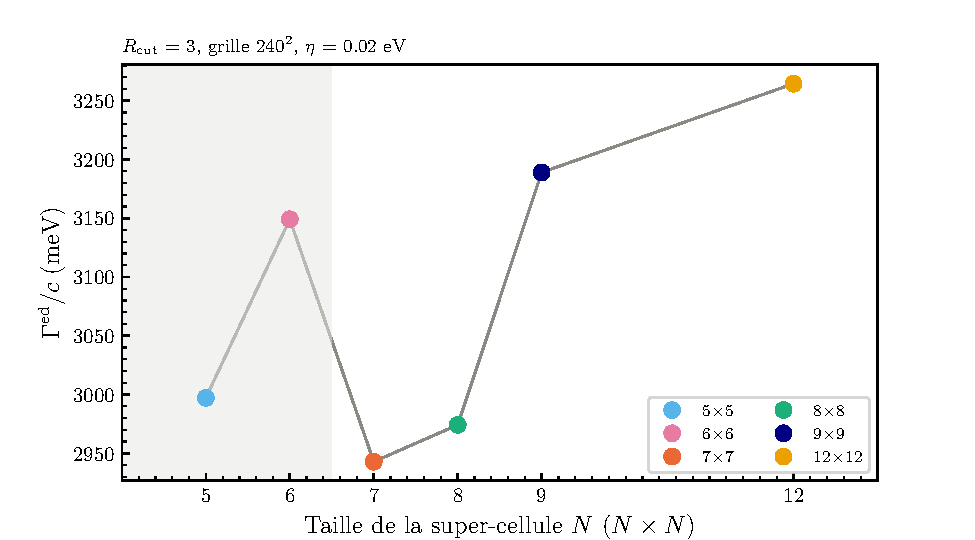
\includegraphics[width=\textwidth]{figures/fig_level2.pdf}
    \caption[Convergence du taux d'amortissement en taille de
    super-cellule.]{Médiane du taux d'amortissement $\Gamma N_\text{cells}$ sur $\pm3$~eV autour de $E_D$ en fonction de la taille $N$ de la super-cellule, avec
    les paramètres de production déterminés~: $R_\text{cut} = 3$, une grille de sortie de $240\times240$, un élargissement $\eta = 20$~meV et une grille interne de $300\times 300$. Les carrés représentent la famille avec $N$ divisible par trois ($N = 3m$) et les ronds représentent l'autre famille.}
    \label{fig:level2}
\end{figure}

Il reste la taille $N$ de la super-cellule, que nous examinons au sein de chaque famille de la section~\ref{sec:M_détails} dans la figure~\ref{fig:level2}. Il est évident que la convergence en taille de la super-cellule n'est pas atteinte, puisqu'aucun plateau n'est présent. Cependant, il y a une réduction régulière d'un facteur de $\sim 2$ par étape qui borne l'erreur de la référence $9\times9$ à $0.6$~\% par rapport à la super-cellule $12\times 12$, ce qui est suffisant pour les conclusions de ce chapitre. Il faudrait effectuer les calculs avec des super-cellules encore plus larges, ce que nous n'avons pas fait faute de temps et de ressources. Cette extension est laissée en perspective.

\newpage
\bloc{Tests du schéma local}

Le tableau~\ref{tab:tests_T} rassemble les vérifications du schéma local de la section~\ref{sec:T_détails}. Le test de référence compare le taux d'amortissement obtenu par le schéma local à celui de l'inversion directe de l'équation~\eqref{eqn:T_chap}, dans le même sous-espace des cinq fonctions de Wannier. Les deux coïncident à $5\times 10^{-14}$ pour $N=5$ et $\sim 10^{-9}$ pour $N=6, 12$. L'évaluation sur la grille d'énergie de pas $\eta/n_e$ introduit, par rapport à une grille quatre fois plus fine ($n_e = 32$), une erreur de $8\times 10^{-4}$ en médiane et de 1.5~\% au pire état. La médiane du taux d'amortissement sur la fenêtre ne change que de $3\times 10^{-4}$. Le taux est positif pour tous les états et $M_\text{loc}$ est hermitienne, comme l'imposent les contrôles. Comme à la section~\ref{sec:M_results}, ces tests établissent la cohérence interne de la méthode. Le contrôle externe vient de la comparaison avec la littérature, que nous effectuons plus bas.
\begin{table}[htbp]
    \centering
    \small
    \setlength{\tabcolsep}{4pt}
    \caption[Vérifications du schéma local.]{Vérifications de la chaîne
    de calcul local de la matrice $T$ et du taux d'amortissement : les tests et la quantité qu'ils contrôlent, la valeur obtenue et le seuil d'acceptation. Le test de
    référence compare le schéma local à l'inversion dense de
    l'équation~\eqref{eqn:T_chap} dans le sous-espace des cinq fonctions
    de Wannier. L'erreur de la grille d'énergie est mesurée par rapport à
    une grille quatre fois plus fine ($n_e = 32$), sur les états de la
    fenêtre $\pm3$~eV de la super-cellule référence $9\times9$. L'écart de la grille interne est mesuré entre $N_{\tilde\kv}=300^2$ et $600^2$ à paramètres de production fixés.}
    \label{tab:tests_T}
    \begin{tabular}{l l l l}
        \hline\hline
        Test & Quantité & Valeur & Seuil \\
        \hline
        Référence, $5\times5$ & $|\Gamma_\text{loc}-\Gamma_\text{dense}|/\Gamma$ & $5.1\times10^{-14}$ & $10^{-8}$ \\
        Référence, $6\times6$ & idem & $6.1\times10^{-9}$ & $10^{-8}$ \\
        Référence, $12\times12$ & idem & $3.7\times10^{-9}$ & $10^{-8}$ \\
        Grille d'énergie, $n_e = 8$ & $|\Delta\Gamma|/\Gamma$, méd. / p95 / max & $8\times10^{-4}$ / $5\times10^{-3}$ / $1.5\times10^{-2}$ & --- \\
        \quad sur la médiane de $\Gamma$ & écart relatif & $3\times10^{-4}$ & --- \\
        Grille interne, $300^2\to600^2$ & écart sur la médiane & $1.4\times10^{-3}$ & --- \\
        Hermiticité de $M_\text{loc}$ & $\max|M_\text{loc}-M_\text{loc}^\dagger|$ & $<10^{-10}$ & $10^{-10}$ \\
        Positivité & $\min\Gamma_{n\kv}$ & $\ge 0$ & $-10^{-8}$ \\
        \hline\hline
    \end{tabular}
\end{table}

\newpage
\bloc{Taux d'amortissement et approximation de Born}

\begin{figure}[htbp]
    \centering
    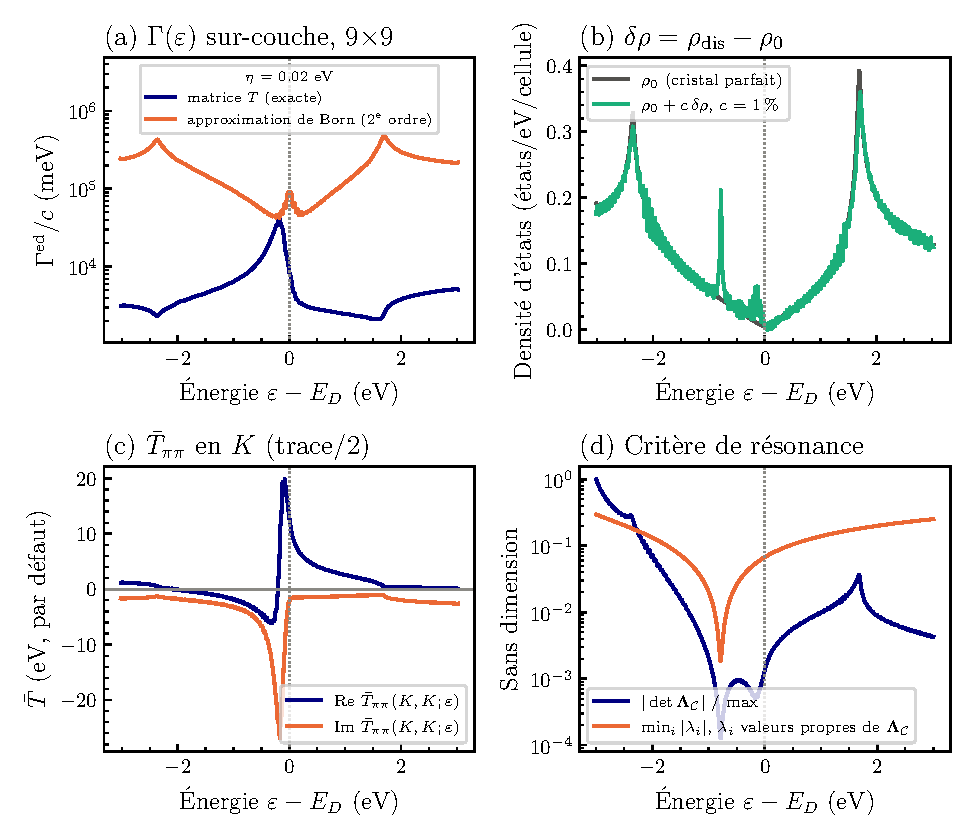
\includegraphics[width=\textwidth]{figures/fig_spectral_final.pdf}
    \caption[Taux d'amortissement et signatures spectrales d'une lacune
    dans le graphène.]{Taux d'amortissement et signatures spectrales d'une lacune dans le graphène, calculés pour la super-cellule de référence $9\times 9$ et les paramètres de production : $R_\text{cut}=3$, la grille de sortie $240\times 240$, un élargissement de $\eta=20$~meV et la grille interne de $300\times 300$. Les énergies sont mesurées à partir du point de Dirac $E_D$. (a) Taux d'amortissement sur couche $\Gamma N_\text{cells}$ des bandes $\pi$ et $\pi^*$ avec la matrice $T$ complète et l'approximation de Born, obtenu par la moyenne lorentzienne~\eqref{eqn:moyenne_lorentzienne} des taux individuels $\Gamma^\text{ed}_{n\kv}$ (b) Densité d'états du cristal parfait $\rho_0$ et pour une concentration de lacunes de $c=1~\%$, $\rho = \rho_0+c\delta\rho$. (c) Parties réelles et imaginaires de la quantité $\bar T(K;\varepsilon)$, définie comme la demi-trace sur la paire $\pi/\pi^*$ dégénérée en $K$, à l'image de $\bar M(K)$ de l'équation~\eqref{eqn:M_bar}. (d) Critère de résonance $\left|\det[\mathbb{I}-M_\text{loc}g^{(0)}(\varepsilon)]\right|$ normalisé et les plus petites valeurs propres de $\mathbb{I}-M_\text{loc}g^{(0)}$.}
    \label{fig:spectral}
\end{figure}
La figure~\ref{fig:spectral} (a) montre le taux d'amortissement $\Gamma N_\text{cells}$ des bandes $\pi$ et $\pi^*$, calculé avec la matrice $T$ complète et l'approximation de Born, pour les paramètres de production déterminés plus haut. Pour passer des taux individuels $\Gamma_{n\kv}^\text{ed}$, évalués chacun à leur propre énergie $\varepsilon_{n\kv}$, à une courbe continue en $\varepsilon$, nous prenons la moyenne lorentzienne normalisée
\begin{equation}
    \Gamma^\text{ed}(\varepsilon) = \frac{\sum_{n\kv}L_\eta(\varepsilon-\varepsilon_{n\kv})\Gamma^\text{ed}_{n\kv}}{\sum_{n\kv} L_\eta(\varepsilon-\varepsilon_{n\kv})},\qquad L_\eta(\varepsilon) = \frac{1}{\pi}\frac{\eta}{\varepsilon^2+\eta^2},\label{eqn:moyenne_lorentzienne}
\end{equation}
sur les états de la grille $240^2$ dans une fenêtre $|\varepsilon-E_D|\leq 3$~eV, avec $\eta=0.02$~eV. Le dénominateur est la densité d'états lisse et $\Gamma^\text{ed}(\varepsilon)$ est le taux d'amortissement moyen des états situés à moins de $\sim \eta$ de $\varepsilon$. Les médianes citées dans les tableaux de convergence sont prises sur les états eux-mêmes ; seule cette figure passe par la moyenne lorentzienne. À $c=1$~\%, le taux exact vaut $\sim 25$~meV en médiane sur la fenêtre de $\pm 3$~eV autour de $E_D$ et est maximal autour de $-1.2$~eV. L'approximation de Born surestime le taux exact d'un facteur de $3.3$ en médiane et jusqu'à $16$ au voisinage des singularités de van Hove, où elle diverge avec la densité d'états tandis que la matrice $T$ sature. C'est l'effondrement de l'approximation de Born pour un potentiel de défaut fort comme une lacune, tel que trouvé dans l'article de référence~\cite{kaasbjergAtomisticMatrixTheory2020}.

\newpage
\bloc{Signatures spectrales de la lacune}

Les panneaux (b-d) de la figure~\ref{fig:spectral} examinent la structure de la matrice $T$ elle-même. La quantité $\bar T(K;\varepsilon)$ au panneau (c), définie comme la demi-trace du bloc de la \textit{self}-énergie de la paire dégénérée à $K$, a une partie imaginaire minimale à $-1.3$~eV et un module maximal entre $-1.05$ et $-0.70$~eV. Les deux parties jouent des rôles distincts. C'est la partie imaginaire qui gouverne l'amortissement : son minimum coïncide avec le maximum de $\Gamma^\text{ed}$ au panneau (a), et non le maximum du module, situé quelque $0.3$~eV plus haut. La région de diffusion résonante est donc celle de la partie imaginaire. La partie réelle, elle, renormalise l'énergie des bandes ; elle porte la signature répulsive de la lacune et reste positive partout dans la fenêtre autour du point de Dirac. Le critère de pôle du panneau (d), qui localise les états liés et quasi-liés induits par le défaut, ne présente qu'une seule quasi-annulation à $\sim-2.5$~eV. La variation de densité d'états au panneau (b) confirme cet état : un pic étroit situé juste sous la singularité de van Hove de la bande $\pi$ à $\sim-2.5$~eV représente un état quasi-lié induit par la lacune, au sein du continuum de la bande. La règle de somme $\int\delta\rho\,d\varepsilon = 0$ sur toute la largeur de bande est satisfaite à moins de 0.06 état près. Au voisinage du point de Dirac, $\delta\rho$ ne présente qu'une faible structure.

\bloc{Comparaison avec la littérature}

Ces signatures se comparent à celles obtenues par Kaasbjerg~\cite{kaasbjergAtomisticMatrixTheory2020}, pour une lacune de carbone dans le graphène, qui trouve un état quasi-lié sous le point de Dirac à $c=1~\%$. L'accord est qualitatif seulement : le signe répulsif du potentiel, l'effondrement de l'approximation de Born et l'ordre de grandeur du taux d'amortissement sont en accord. Toutefois, la position exacte de l'état quasi-lié diffère : dans nos calculs, l'état dominant se trouve sous la singularité de van Hove plutôt qu'au voisinage du point de Dirac, où la littérature sur la monolacune du graphène situe le mode quasi-nul~\cite{pereiraDisorderInducedLocalized2006}, et où notre $\delta\rho$ n'a qu'un poids faible. Il est clair que la différence d'un facteur de $3$--$4$ entre nos éléments de matrice, qui se propage non linéairement au taux d'amortissement, a un impact sur cette comparaison quantitative. Nous n'avons pas pu lui attribuer une cause unique parmi la relaxation de la super-cellule défectueuse, le traitement des électrons de c\oe ur, la base d'ondes planes contre celle d'orbitales atomiques, la fonctionnelle d'échange-corrélation et l'approximation diagonale en bande de la matrice $T$ (section~\ref{sec:mbt_sigma}), que la référence n'effectue pas. De plus, nous avons relevé que notre taux n'est pas convergé par rapport à la taille de la super-cellule, ce qui a nécessairement un impact sur les propriétés spectrales de la lacune. Enfin, l'interpolation de la matrice de couplage dans le sous-espace des cinq fonctions de Wannier introduit une approximation : les états au-delà de la fenêtre externe, ainsi que la partie des bandes de haute énergie non capturée par le désenchevêtrement, sont absents de la base dans laquelle la matrice $T$ est construite. Nous nous attendons à ce que ces états ne contribuent pas significativement à la diffusion Raman résonante, mais cela constitue toutefois une différence réelle avec la base d'orbitales atomiques de la référence.

\section{Conclusion}
Ce chapitre a construit, à partir des premiers principes, une méthode complète pour le couplage électron-défaut, qui constitue la contribution originale centrale de ce mémoire. Les éléments de matrice $M_{mn}(\kv',\kv)$ sont définis à partir du potentiel induit par le défaut et séparés en une partie locale, évaluée dans l'espace réciproque~\eqref{eqn:ML_final}, et une partie non locale issue des projecteurs de Kleinman-Bylander~\eqref{eqn:MNL_final}. Deux idées centrales rendent notre méthode applicable au calcul de l'intensité Raman résonante sur des grilles ultra-denses. D'abord, le remplissage par zéros raffine la grille du potentiel de défaut et allège la contrainte de commensurabilité entre la super-cellule et la grille des fonctions de Wannier, ce qui nous permet d'obtenir la matrice de couplage sur des grilles relativement denses sans recourir à des calculs de super-cellules démesurés et intraitables. Ce remplissage par zéros rend par ailleurs manifeste la localisation des éléments de matrice de couplage dans la base de Wannier (section~\ref{sec:M_results}), ce qui autorise notre deuxième idée : l'interpolation par fonctions de Wannier, tronquée à un sous-espace local de petite dimension grâce à cette localisation, qui rend le calcul de la matrice $T$ praticable sur des grilles arbitrairement denses.

Nous avons appliqué notre méthode à une lacune non relaxée dans le graphène et ce chapitre livre trois résultats principaux. D'abord, l'échantillonnage de la zone de Brillouin sépare les super-cellules en deux familles selon que leur grille inclut ou non les points $K$ et $K'$ et nous prenons la super-cellule $9\times 9$, dont la grille les inclut, comme référence. Ensuite, le couplage est dominé par sa partie non locale, tandis que la partie locale, écrantée, porte toute la dépendance en taille de la super-cellule. Enfin, le taux d'amortissement par unité de concentration, obtenu dans le formalisme de la matrice $T$, révèle un état quasi-lié sous la singularité de van Hove de la bande $\pi$, plus profond que le mode quasi-nul attendu près du point de Dirac selon la littérature. L'approximation de Born surestime ce taux et diverge aux singularités de van Hove : pour un potentiel aussi intense que celui d'une lacune, la resommation de la matrice $T$ à tous les ordres en théorie de la perturbation est nécessaire. La chaîne de calcul est validée par une suite de tests systématiques, dont la reconstruction des valeurs propres de Kohn-Sham à quelques dizaines de $\mu$eV près.

Notre méthode souffre toutefois de plusieurs limitations. La géométrie autour du défaut n'est pas relaxée et la reconstruction de Jahn-Teller de la monolacune~\cite{el-barbaryStructureEnergeticsVacancy2003} est ignorée. Le taux d'amortissement n'est convergé qu'à $0.6$~\% entre les super-cellules $9\times 9$ et $12\times 12$, sans qu'un plateau soit atteint mais avec une décroissance régulière des écarts. Nos éléments de matrice calculés sont inférieurs d'un facteur de $3$--$4$ à ceux de Kaasbjerg~\cite{kaasbjergAtomisticMatrixTheory2020}, sans qu'une cause unique ait pu être isolée parmi la fonctionnelle d'échange-corrélation, la base d'ondes planes plutôt que d'orbitales atomiques, la relaxation autour du défaut, le traitement des électrons de c\oe ur, la troncature du sous-espace des fonctions de Wannier et l'approximation diagonale en bande de la matrice $T$. L'accord des éléments de matrice et des signatures spectrales reste toutefois qualitatif. La relaxation de la lacune, la généralisation à d'autres types de défauts, la convergence en taille de la super-cellule du taux d'amortissement, l'approximation de la matrice $T$ autocohérente au voisinage du point de Dirac~\cite{peresElectronicPropertiesDisordered2006}, ainsi que la structure matricielle en bande complète de la matrice $T$ sont laissées en perspective. De surcroît, nos calculs ne sont pas polarisés en spin, alors que la monolacune du graphène porte un moment magnétique local~\cite{yazyevDefectinducedMagnetismGraphene2007}. Un traitement polarisé, couplé à la relaxation de Jahn-Teller, modifierait la position de l'état quasi-lié et séparerait le taux d'amortissement en deux contributions de spin. Enfin, nous ne considérons qu'un seul type de défaut dans ce mémoire : les lacunes. La méthode est toutefois généralisable à n'importe quel type de défaut et cette généralisation est elle aussi laissée en perspective.

Le chapitre livre ainsi les deux quantités annoncées en introduction. Les éléments de matrice $M$ entrent directement dans les amplitudes de diffusion \textit{phonon-défaut} du chapitre~\ref{chap:Raman} et le taux d'amortissement $\Gamma^\text{ed}$ élargit les dénominateurs résonants de ces amplitudes. Pour les énergies d'excitation dans le visible typiquement utilisées dans les expériences de spectroscopie Raman, les états intermédiaires de la double résonance se situent précisément dans la fenêtre d'énergie où la diffusion sur la lacune est maximale et où l'approximation de Born échoue le plus~\cite{thomsenDoubleResonantRaman2000}. Le chapitre suivant calcule le second ingrédient de ces dénominateurs, le taux d'amortissement dû au couplage électron-phonon $\Gamma^\text{ep}$, et nous verrons que les deux contributions sont comparables dans cette fenêtre.